\section{Números}
Para los números se arma por partes, tomando el conjunto de los dígitos
	$$d = [0,9] = {0,1,2,\ldots ,9},$$
se arman los números enteros con la clausura positiva, para asegurar que entre al menos un dígito, parte entera
	$$d^+;$$
ahora, tomando la parte de los reales, es necesario agregar el punto decimal y otra sucesión de dígitos que contenga al menos a uno de ellos
	$$d^+ .d^+,$$
la primera parte del condicional da los reales y la segunda parte es simplemente para continuar con el número de entero. Para los complejos solo se agranda la expresión sumandole una igual con la unidad imaginaria añadida
	$$d^+ \qty(.d^+ |d^*) \qty(+|-) d^+ \qty(.d^+ |d^*)i.$$
Para los númreros en notación científica se utilizó la notación con la letra $E$; es decir, $6.67E-11$. Para ello, se construyó la expresión regular
	$$(d^+|d^+.d^+)E(d^+|-d^+).$$




\section{Fecha}
Para los tres formatos de fecha, se tomarán los intevalos de enteros:
\begin{align*}
	\left\{\begin{array}{c}
		d \in [1,31] \\
		m \in [1,12] \\
		a_1 \in [00,99] \\
		a_2 \in [1000,9999]
	\end{array}\right.
\end{align*}
Dados los formatos, no se tomarán años, anteriores a los $1000$ d.c. ni posteriores a los $1000$ a.c. Dado esto, la expresión regular es
\begin{align*}
	\Aboxed{d\qty(/m/(a_1|a_2)|-m-(a_1|a_2))}
\end{align*}
Se coloca de este modo, para no combinar formatos, es decir, que la fecha $17/12-2000$ no sea aceptada.





\section{AFDs}
Los automatas finitos determinstas encontrados mediante el método de Thompson, son: (Para los números complejos, se crearon dos automatas, uno para donde las partes real e imaginaria son enteras y otro para cuando son reales; esto porque un despiste y falta de tiempo.)
\begin{multicols}{2}
\begin{description}
	\item[Enteros: ] AFD:
		\begin{figure}[H]
			\centering
			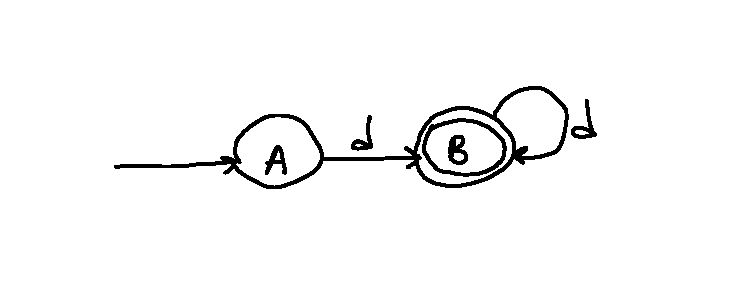
\includegraphics[scale=0.65]{Images/AFDenteros.pdf}
			\caption{AFD generado para los números enteros.}
			\label{fig:enteros}
		\end{figure}
	\item[Reales: ] AFD:
		\begin{figure}[H]
			\centering
			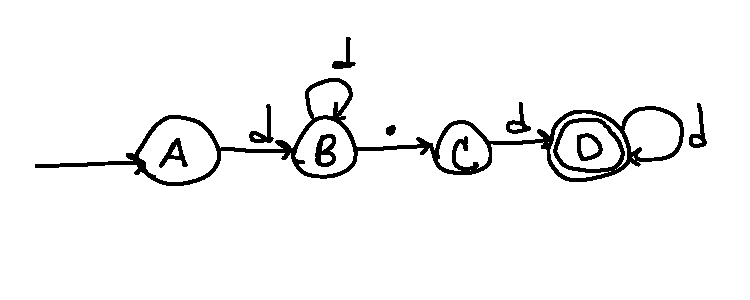
\includegraphics[scale=0.65]{Images/AFDreales.pdf}
			\caption{AFD generado para los números reales.}
			\label{fig:reales}
		\end{figure}
	\item[Complejos: ] AFD:
		\begin{figure}[H]
			\centering
			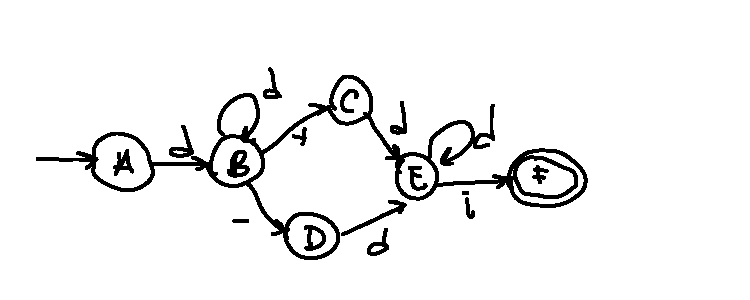
\includegraphics[scale=0.65]{Images/AFDcomplejosenteros.pdf}
			\caption{AFD generado para los números complejos con partes enteras.}
			\label{fig:complejose}
		\end{figure}
		\begin{figure}[H]
			\centering
			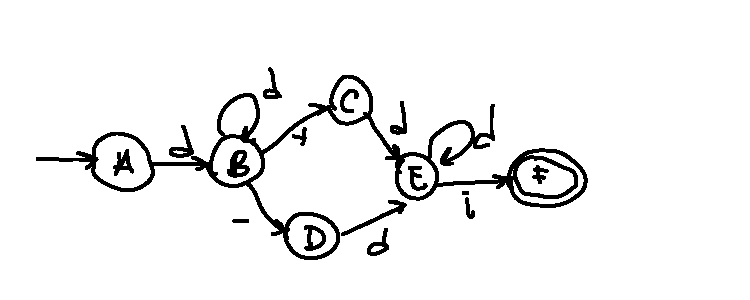
\includegraphics[scale=0.65]{Images/AFDcomplejosenteros.pdf}
			\caption{AFD generado para los números complejos con partes reales.}
			\label{fig:complejosr}
		\end{figure}
	\item[Notación Científica: ] AFD:
		\begin{figure}[H]
			\centering
			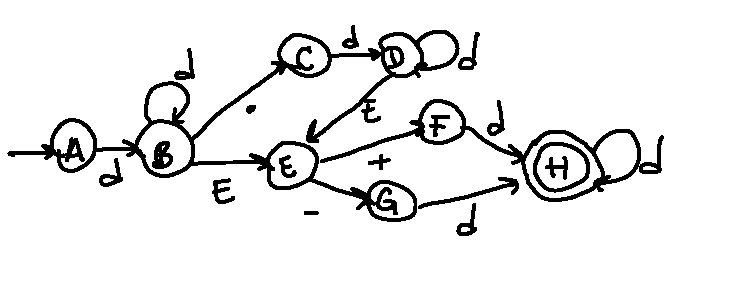
\includegraphics[scale=0.65]{Images/AFDnotacioncientifica.pdf}
			\caption{AFD generado para los números escritos en notación científica.}
			\label{fig:notacioncientifica}
		\end{figure}
	\item[Fechas: ] AFD:
		\begin{figure}[H]
			\centering
			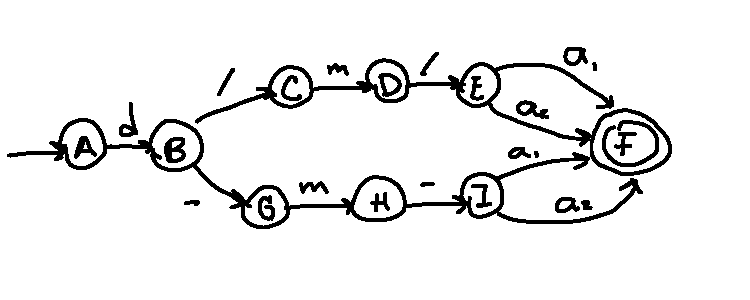
\includegraphics[scale=0.65]{Images/AFDfechas.pdf}
			\caption{AFD generado para las fechas en formato $dd/mm/aaaa$ y $dd-mm-aaaa$.}
			\label{fig:fechas}
		\end{figure}
\end{description}
\end{multicols}






\section{Palabras Clave}
La expresión regular utilizada para las palabras clave es simple, únicamente se toman ambos conjuntos de palabras y se colocan en union:
	$$\qty(\text{Teorema}|\text{Matemática}|\ldots |\text{Experimentación}| \text{Físico}|\ldots),$$

en donde todas las palabras llevan a estados de aceptación. Estas palabras, se tomarán en cuenta, incluso si no contienen la inicial mayuscula.























